\chapter{Methodology}

A methodology for achieving security, scalability, and resource distribution in a cloud-native architecture is described in this chapter. The approach integrate different architectures to address specific research objectives and requirements. The primary objective of this research is the development of an architecture that provide secure, scalable and distributed computing platform. To achieve this objective, a combination of cloud-native technologies and tools are used, particularly in the context of AI model deployment.

\section{Authentication}

In a cloud-native architectures, authentication is the foundation for securing access to resources. Authentication provides protection of shared information from unauthorized access. It is essential for maintaining data security. Authentication methods are designed in a way that can verify the identity of users and confirm that they are who they claim to be and determine whether they are authorized to access sensitive information. In a cloud-native architectures, where multiple services and applications interact with each other, it become crucial to provide authentication mechanism to streamline access and maintain security. By implementing a secure SSO mechanism using authentication protocols, we can effectively authenticate users and enhance overall security. \cite{babaeizadeh2015authentication}

\subsection{Single Sign-On}

SSO is a cloud-native identity and access management solution in cloud-native architecture that enhance the security of the application and or user experience by centralizing the authentication system. SSO allows users to log in with a single set of credentials and then use many secure resources without having to log in again and also helps to reduce the number of passwords that users need to remember to access different applications, making it much more efficient and secure. SSO helps reduce the number of accounts, the administrative burden of managing user privileges and the likelihood of privilege violations. Implementing SSO with OIDC and OAuth helps to authenticate users and improve security by combining access management into a single, manageable framework. \cite{babaeizadeh2015authentication}

\subsection{Authentication Protocol}

Authentication protocols are essential for implementing SSO, as they provide standardised methods for managing user authentication and authorization across different applications. Commonly used protocols include OAuth2, SAML and OpenID, each of which plays an important role in improving security and streamlining access. OAuth is an open authorization protocol that enables secure access to resources by issuing tokens rather than using traditional username and password methods. SAML facilitate communication between identity providers and service providers with regards to SSO using different authentication methods, it is one of the core components of cross domain SSO implementation frameworks.. OpenID, on the other hand, allows users to authenticate without relying on a central server and uses identifiers, trusted parties and providers to manage user authentication and verification processes. The using these protocols, the aim is to create an SSO mechanism that simplifies user access and improves overall security in our cloud-native architecture. \cite{waluyo2022comparative}

\section{Authorization and Access Control}

Once a request has been authenticated, it moves on to the authorization phase, which is a critical part of securing Kubernetes clusters, ensuring that only authenticated users and services with the appropriate permissions can interact with cluster resources. This involves verifying whether a user or service is allowed to perform a specific action on a specific resource. This process is used to hold security and prevent intrusion since it adheres to certain policies that determine potential security risks and actions to avoid those risks, by protecting potentially vulnerable areas in cloud-native architectures. \cite{zahoor2023formal}

Access control is the mechanism used to grant permissions within the cluster. In Kubernetes, The RBAC system allows to control access to resources in a more granular manner through building different levels of permissions and policies. This system regulates the actions that users and service accounts are allowed to perform, ensuring that only authorized entities can access and interact with critical resources. To enhance the security of our Kubernetes cluster in a cloud-native architectures, we will implement RBAC as a fundamental component of our access control strategy. \cite{mustyala2021advanced}

\section{Distributed Computing Framework}

Distributed computing frameworks are critical components of cloud-native architectures that enable efficient processing of large amounts of data on clusters or in the cloud. Their main purpose is to distribute computing work across multiple computers, reducing the load and potential risks of concentrating computing on a single computer and providing high scalability, reliability, manageability and flexibility. As the size and complexity of AI models grow faster than the computing power of clusters, traditional distributed computing frameworks based on the MapReduce model are insufficient to support AI tasks. These tasks often involve running complex analytical algorithms on large-scale AI models with billions of parameters. However, existing frameworks face key challenges such as computational inefficiency, limited scalability due to memory constraints, and limited algorithmic capabilities because many sequential algorithms cannot be implemented within the MapReduce programming model. Therefore, new distributed computing frameworks are needed to address these challenges. This research utilized a flexible distributed computing framework with the potential to overcome the challenges of AI model analysis and provide autoscaling to ensure resource scalability. \cite{sun2023survey, chen2023advance}

\subsection{Optimization of AI Models}

Optimising AI models at scale requires the use of distributed computing frameworks due to the significant complexity and size of modern machine learning problems. As data volumes and model complexity continue to escalate, with datasets ranging from 1TB to 1PB and models containing between $10^9$ and $10^{12}$ parameters, it becomes impractical for a single machine to perform the required computations efficiently. Distributed optimization frameworks are essential to deal with these challenges on a large-scale. In a distributed setup, both data and computational workloads are distributed across multiple worker nodes. These nodes collaborate by frequently accessing and updating shared parameters, which can be represented as dense or sparse vectors and matrices. The distributed framework handles the asynchronous data communication between nodes for the purpose of maintaining consistency of the global parameters across all workers. This approach supports various consistency models enabling further control of data consistency and synchronization. By using distributed computing, optimization can solve fundamental problems of large and complex ML and DL models and improve the training process of large-scale AI models. \cite{li2014scaling}

\subsection{Scalability of Resources}


Scalability is an apt feature in distributed computing frameworks like Kubernetes cluster that is used for handling dynamic workloads to achieve efficient resource utilization. The resource scaling is
normally done with regards to the number of replicas of any workload or the number of replicas modified with respect to the ratio between the current metric value as well as the target metric value. The formula used to calculate for the number of replicas needed is

\[
\text{desiredReplicas} = \left\lceil \text{currentReplicas} \times \left( \frac{\text{currentMetricValue}}{\text{desiredMetricValue}} \right) \right\rceil
\]


This equation calculate and adjust with the number of replicas depending on workload such as when the current value is two times the desired metric, the system will set the number of replicas equal to multiple of two to the current metric value. On the other hand, if the current load is cuts down to half of its required value, the number of replicas is also halved. The scaling action is isolated if the current and the corresponding desired value is close enough to a small and adjustable tolerance thus avoiding unnecessary scaling actions, even if the values are not optimal. It is one of the scalability techniques that control the computing resources considering the changes of workload, it can provide dynamic allocation of resources which in result helps to control the performance and prevent waste of resources. Due to their ability to scale up or down, and distribute the work, distributed frameworks are more reliable and adaptable to the changing conditions and to achieve best performance by the use of dynamic computing resources. \cite{Kubernetes_doc}


\clearpage



\autoref{fig:Secure and Scalable} below illustrates the secure, scalable and distributed computing architecture using
distributed computing framework to implement authentication and authorization to achieve a secure, scalable, and distributed computing architecture that is capable of deploying the AI model.

\begin{figure}[h]
\centering
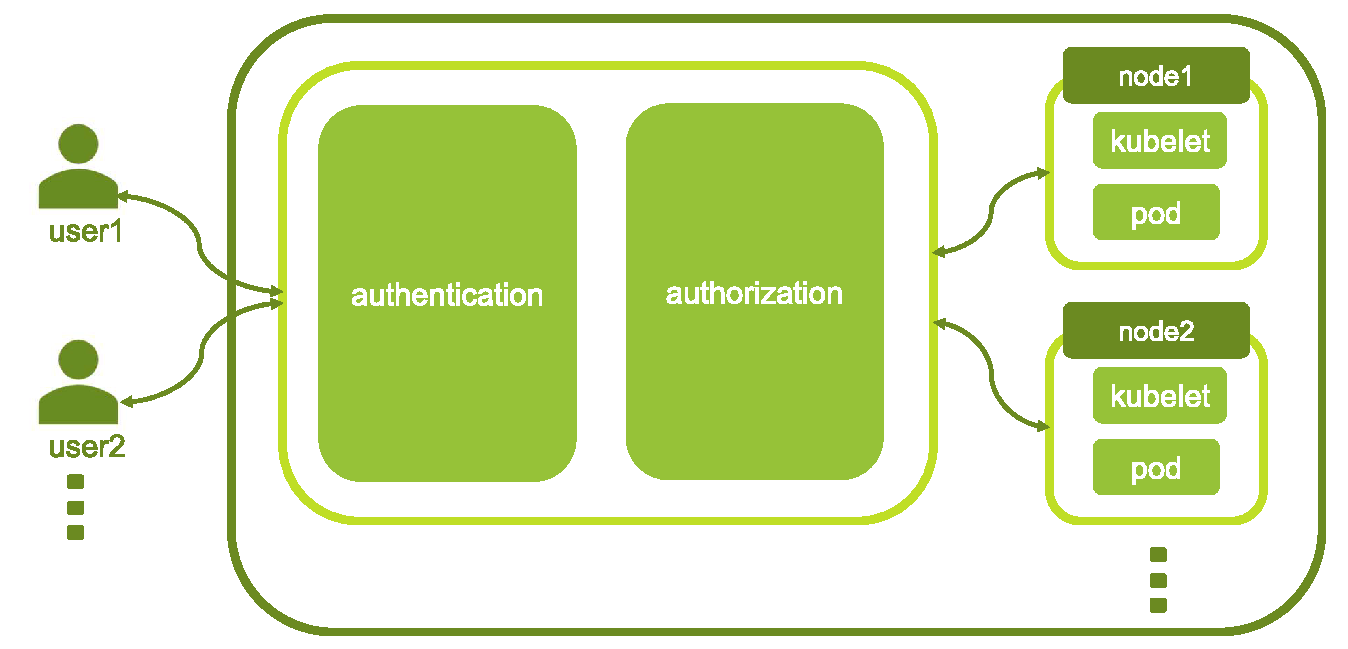
\includegraphics[width=1 \linewidth]{Thesis/Figures/Slide47.pdf}
\caption{\label{fig:Secure and Scalable}Secure and Scalable Architectures}
\end{figure}

